\documentclass[a4paper,titlepage,11pt]{article}

\usepackage[top=2.54cm, bottom=2.54cm, left=2.54cm, right=2.54cm]{geometry}
\usepackage[utf8x]{inputenc}
\usepackage{hyperref}
\usepackage{graphicx}
\usepackage{hyperref}
\usepackage{multicol}
\usepackage{textcomp, xspace}

\begin{document}

\begin{titlepage}
  \begin{center}
    {\scshape \huge Schelling's Model of Segregation \par}
    \vspace{1cm}

    {\scshape \LARGE Project \par}
    \vspace{1.5cm}

    {\scshape \Large Complex Network \par}
    \vspace{0.5cm}

    {\Large Alameda \par}
    \vfill

    {\itshape \Large Group 6 \par}
    \vfill

    \begin{tabular}{l l}
      Bernardo Casaleiro & 87827\\
      João Godinho & 87830\\
    \end{tabular}
    \vfill

    {\large \today\par}
  \end{center}
\end{titlepage}

\section{Introduction}
For this project we had to create and analyze the Schelling's Model. This model has the purpose of studying the segregation of races over time showing that when agents don't mind being surrounded by agents of a different race, they will yet aggrupate themselves from other agents over time.

Our main purpose is to discover the threshold where there is an high or low segregation level.

For this project we decided to continue to use the same language as our first project, so we used \href{https://www.python.org}{Python}. To build the interface we used \href{https://wiki.python.org/moin/TkInter}{Tkinter}, and to draw the graphs (contour plot) we used \href{https://plot.ly/}{plotly}.

\section{Implementation}

\subsection{Heuristics}
There were three heuristics created: Random, Best, Closest.

\subsubsection{Random}
In this Heuristic an agent is randomly placed on an empty space.

\subsubsection{Best}
In this heuristic an agent is placed on an empty space where he will be satisfied.

\subsubsection{Closest}
In this heuristic an agent is placed on the closest empty space. In order to avoid that an agent is always switching between two spaces, each agent has a memory that keeps track of the last empty space he has been to.

\subsection{Variables}
In our interface is possible to change all variables necessary to run the simulation:

\textit{ \textbf{Interface Variables} }

\begin{figure}[h]
    \centering
    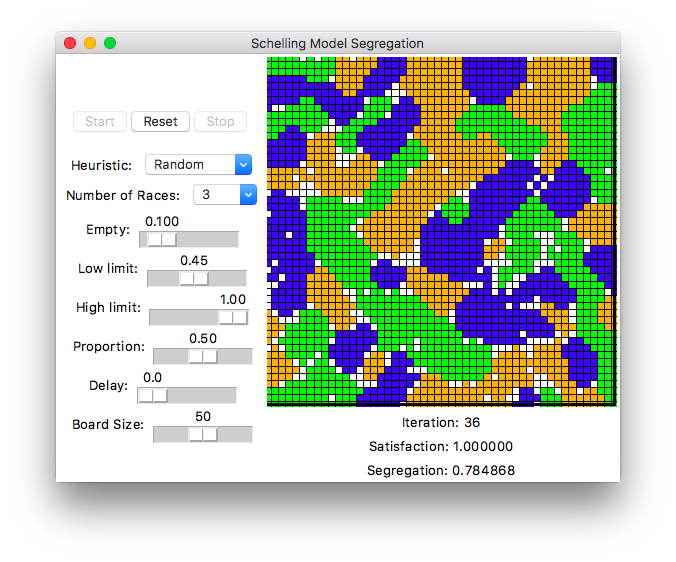
\includegraphics[scale=0.50]{img/interface.png}
\end{figure}

\begin{description}
\item [ Heuristic ] (Random or Best or Closest) \textbf{-} heuristic used for simulation
\item [ Number of Races ] (2 or 3) \textbf{-} number of races there will exist
\item [ Empty ] (0.0-1.0) \textbf{-} percentage of empty spaces
\item [ Low limit ] (0.0-1.0) \textbf{-} minimum level of satisfaction
\item [ High limit ] (0.0-1.0) \textbf{-} maximum level of satisfaction
\item [ Proportion ] (0.0-1.0) \textbf{-} proportion between the number of agents in each race, when number of races equals 2
\item [ Delay ] (0.0-2.0) \textbf{-} time between each iteration
\item [ Board Size ] (0-100) \textbf{-} size of the simulation board
\end{description}

\section{Results}

\section{Reference}

\end{document}
